% !TeX spellcheck = en_US
\chapter{Implémentation d'un système multi-agents avec la plateforme JADE}
\section{Outils utilisés}
\section{Schéma globale}
\paragraph{}
Notre conception du système multi-agents se base sur trois types d’agents:

Agent central: c’est l’agent qui s’occupe de la gestion des centres de ventes, il reçoit les requêtes des utilisateurs, après traitement il leur retourne les produits qu’ils cherchent.

Agent annexe: représente les vendeurs. Il reçoit une requête de l’agent central et il lui remet les produits présents dans sa base de données qui correspondent  à la requête.

Agent enregistreur: c’est l’agent qui garde les informations sur les différents agents centraux et annexes.
\newpage
\subsection{Agent annexe}
\paragraph{}
L’agent annexe se charge non seulement de répondre aux requêtes émises  par les centres de ventes mais aussi d’inférer des attributs à partir des informations de la requête pour mieux répondre à cette dernière.

Chaque agent annexe a une liste de règles qui permettent à un système expert de savoir si cet agent peut posséder un produit donnée.
\begin{figure}[H]
	\centering
	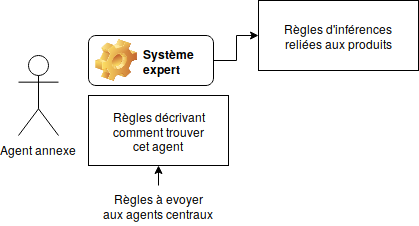
\includegraphics[scale=0.75]{imgs/annexeAgent.png}
	\caption{Illustration de l'agent annexe}
	\label{fig:annexeAgent}
\end{figure}

\subsection{Agent central}
\paragraph{}
L’agent central reçoit d’abord les règles des agents annexes afin qu’il puissent par la suite les contacter après avoir reçu une requête de l’utilisateur.
\begin{figure}[H]
	\centering
	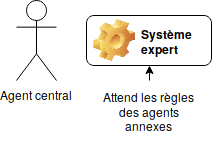
\includegraphics[scale=0.75]{imgs/centralAgent.png}
	\caption{Illustration de l'agent central}
	\label{fig:centralAgent}
\end{figure}


\section{Communication entre les agents}
La communication entre les agents se devise en deux parties principales:
\begin{itemize}
	\item Communication d’ajout de service.
	\item Communication de requête.
\end{itemize}
\subsection{Communication d'ajout de service}
Ce type de communication est principalement géré par l’agent enregistreur. Tout agent qui arrive dans le système devra  informer un agent enregistreur pour qu’il puissent garder ses informations.
\begin{figure}[H]
	\centering
	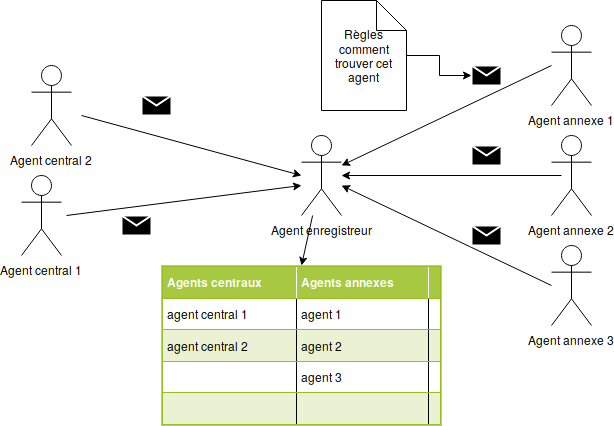
\includegraphics[scale=0.6]{imgs/comReg.png}
	\caption{Enregistrement des agents}
	\label{fig:registrations}
\end{figure}
Par la suite, l’agent enregistreur répond aux agents centraux et il leur communique les règles concernant les agents annexes afin qu’ils puissent les trouver lors de l’arriver d’une requête utilisateur.
\begin{figure}[H]
	\centering
	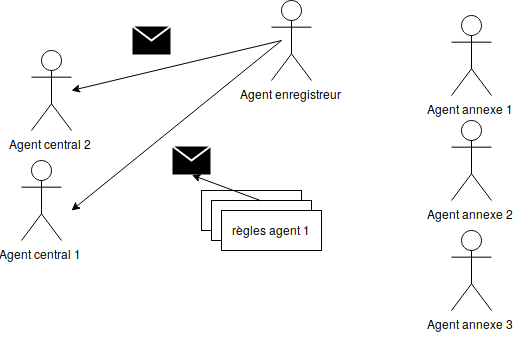
\includegraphics[scale=0.6]{imgs/sendRules.png}
	\caption{Enregistrement des agents}
	\label{fig:comRules}
\end{figure}
\newpage
Jusqu’à présent le vrai rôle de l’agent enregistreur n’apparait pas. C’est quand un nouveau agent qui se connecte dans le système qu’on aperçoit son rôle. Le nouveau agent n’a pas à communiquer avec tous les autres agents pour qu’il soit connu dans son environnement, il suffit d’informer l’agent enregistreur pour réaliser cela. Quand un agent annexe arrive, il envoi ses informations à l’agent enregistreur, ce dernier informe les agents centraux de son arrivé pour qu’ils puissent le contacter.
\begin{figure}[H]
	\centering
	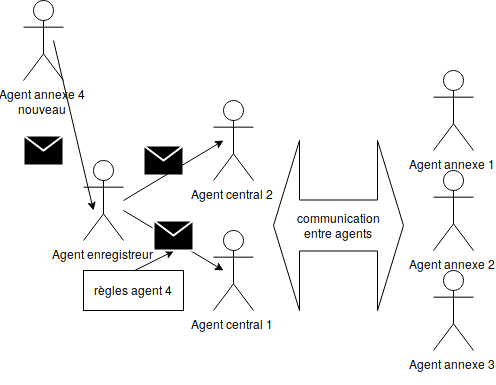
\includegraphics[scale=0.6]{imgs/newAnnexe.png}
	\caption{L'arrivé d'un nouveau agent annexe}
	\label{fig:newAnnexe}
\end{figure}
Quand un agent central arrive, l’agent enregistreur l’informe des agents annexes existant, et l’ajoute à la liste des agents centraux.
\begin{figure}[H]
	\centering
	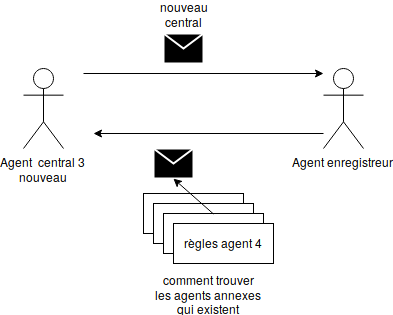
\includegraphics[scale=0.6]{imgs/newCentral.png}
	\caption{L'arrivé d'un nouveau agent central}
	\label{fig:newCentral}
\end{figure}
\newpage
\subsection{Communication de requêtes}
Ce type de communication concerne la partie des communications qui résulte de l’arriver d’une requête utilisateur. L’agent central qui reçoit la requête lance son moteur d’inférence pour déduire les agents susceptible d’avoir les produits spécifié par la requête. La requête est alors envoyer à ces agents pour qu’ils puissent y répondre.
\begin{figure}[H]
	\centering
	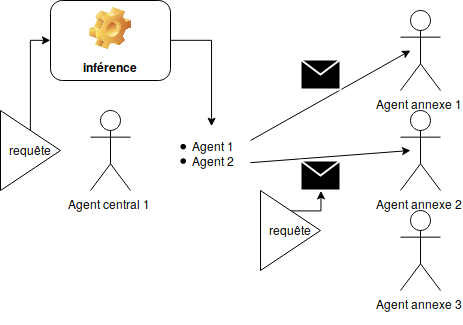
\includegraphics[scale=0.6]{imgs/annexeSelec.png}
	\caption{La sélection des agents annexes}
	\label{fig:annexeSelection}
\end{figure}
L'agent annexe qui reçoit la requête commence d’abord par essayer d’inférer de nouvelles connaissances sur le produit que l’utilisateur cherche. Ensuite il cherche dans sa base de données les produits qui correspondent à la requête. Le résultat obtenu est retourner à l’agent central pour qu’il les propose à l’acheteur.
\begin{figure}[H]
	\centering
	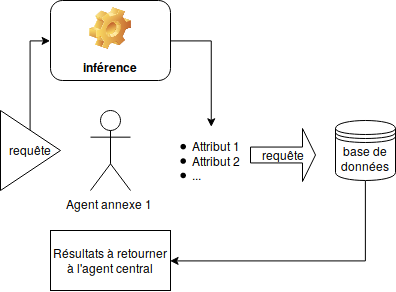
\includegraphics[scale=0.6]{imgs/annexeWork.png}
	\caption{Le travail d'un agent annexe}
	\label{fig:annexeWork}
\end{figure}

%amaze me here